\documentclass[10pt]{beamer}

\usetheme{Montpellier}
\usecolortheme{whale}

\usepackage[T1]{fontenc}
\usepackage{lmodern}

\usepackage{mathtools}
\usepackage[binary-units]{siunitx}
\usepackage{amsmath}
\usepackage{listings}
\usepackage{mdframed}
\usepackage{adjustbox}
\usepackage{minted}
\usepackage{xcolor}

\usepackage{parskip}
\usepackage{substr}
\usepackage{hyperref}
\usepackage{etoolbox}
\usepackage{tipa}
\usepackage{cprotect}
\usepackage{booktabs}
\usepackage{silence}
\usepackage[backend=biber, style=ieee]{biblatex}
\usepackage[english,ngerman]{babel}
\usepackage{csquotes}

\definecolor{lg}{gray}{0.95}
\hypersetup{colorlinks = true, urlcolor=blue, linkcolor=white}
\WarningFilter{biblatex}{Patching footnotes failed}

\renewcommand*{\bibfont}{\tiny}
\renewcommand{\subsectionname}{AA}

\bibliography{resources.bib}

\title{\textbf{Operating Systems}}
\subtitle{Tutorial 2}
\author{Fabian Klopfer}
\date{\today}

\defbeamertemplate{subsection page}{mine}[1][]{%
  \begin{centering}
    {\usebeamerfont{subsection name}\usebeamercolor[fg]{subsection name}#1}
    \vskip1em\par
    \begin{beamercolorbox}[sep=12pt,center]{part title}
      \usebeamerfont{subsection title}\insertsubsection\par
    \end{beamercolorbox}
  \end{centering}
}

\defbeamertemplate{section page}{mine}[1][]{%
  \begin{centering}
    {\usebeamerfont{section name}\usebeamercolor[fg]{section name}#1}
    \vskip1em\par
    \begin{beamercolorbox}[sep=12pt,center]{part title}
      \usebeamerfont{section title}\insertsection\par
    \end{beamercolorbox}
  \end{centering}
}

\setbeamertemplate{section page}[mine]
\setbeamertemplate{subsection page}[mine]

\begin{document}
\frame{\titlepage}


\begin{frame}{Intro}
\begin{itemize}
 \item Again: Sheet 1 Ex. 4 (FDE Pipeline): \\
 If in the exam, will be asked for the throughput specifically.
 \item Pingo Polls
\end{itemize}
\end{frame}

\section*{Exercise Sheet 3}
\frame{\sectionpage}
\subsection*{Exercise 1}
\frame{\subsectionpage}
\begin{frame}[allowframebreaks, fragile]{Exercise 1}
    \begin{enumerate}
		\item What is the difference between cooperative and preemptive scheduling? \\
		\alert{Cooperative: Scheduler doesn't actively interrupt process; process \textbf{yields}. \\
		Preemptive: Scheduler queues timer interrupt to pause execution and schedule sth. else.}
		\item Name one disadvantage of cooperative scheduling. \\
		\alert{If CPU not released by programmer $\Rightarrow$ System deadlocked}
		\item Which information is required for Shortest-Job-First-Scheduling? \\
		\alert{(Expected) runtime of jobs to schedule.}
		\item If the costs for a context switch are high, should one choose a small or a large time quantum? \\
		\alert{Large to minimize overhead.}
	\end{enumerate}
\end{frame}

\subsection*{Exercise 2}
\frame{\subsectionpage}
\begin{frame}[allowframebreaks, fragile]{Exercise 2}
\begin{enumerate}
		\item% 
            Round Robin: \\
			What could be the use of having a process appear multiple times in the list? \\
			Which problem could occur? \\
			\alert{Prioritization \\
                    If prioritized process blocks, all entries need removal, else blocks CPU.}
                    \framebreak
		\item%
			$H$ (high priority), $L$ (low priority) processes. \\
			$L$ reserves a resource, $H$ becomes ready \& tries to access same resource. \\
			$H$ (actively) waits for $L$ to release the resource, $L$ never receives computing time while $H$ is running and cannot release resource.\\ $\Rightarrow$ Deadlock. \\
			Can this problem also occur if Round-Robin scheduling is used instead of priority scheduling? \\
			\alert{No. $L$ will still get CPU time \& release resource s.t. $H$ can execute.}
	\end{enumerate}
\end{frame}

\subsection*{Exercise 3}
\frame{\subsectionpage}
\begin{frame}[allowframebreaks, fragile]{Exercise 3}
    Avg. process CPU time before IO $T$, context switch takes $S$, Round-Robin scheduling with time quantum~$Q$. \\ Specify formula for CPU efficiency in the following cases.
	\begin{enumerate}
		\item $Q > T$ \\
		\alert{\[\frac{T}{(S+T)}\]
		Process runs until it's doing IO, context switches only happen on IO.}
		\item $S < Q < T$ \\
		\alert{\[\frac{T}{T + S \cdot T/Q}\]
		Requires $\frac{T}{Q} - 1$ context switches due to scheduling $+ 1$ for IO}
		\framebreak
		\item $Q = S$ \\
		\alert{\[ \frac{T}{T + S \cdot T/Q} \Rightarrow \frac{T}{T + Q \cdot T/Q} = \frac{1}{2}\]}
		\item $Q \rightarrow 0$ \\
		\alert{\[ \lim_{Q \rightarrow 0} \text{Context switches share} \rightarrow 100\%\]
		\[\Rightarrow \lim_{Q \rightarrow 0} \text{CPU efficiency} \rightarrow 0\% \]}
	\end{enumerate}
\end{frame}

\subsection*{Exercise 4}
\frame{\subsectionpage}
\begin{frame}[allowframebreaks, fragile]{Exercise 4}
\begin{columns}
\begin{column}{0.6\textwidth}
		\raggedright
		Jobs $A, \ldots, E$. \\
		Determine the average turnaround time for:
		\begin{enumerate}
		\item Round-Robin
		\item Priority
		\item First-Come-First-Serve.\\
		Order: $A$, $B$, $C$, $D$, $E$.
		\item Shortest-Job-First.
	\end{enumerate}
	\end{column}%
	\begin{column}{0.4\textwidth}
		\scalebox{0.8}{
		\begin{tabular}[t]{p{0.3\textwidth} p{0.3\textwidth} p{0.3\textwidth}}
			\toprule
			 Process & Runtime  & Priority \\ 
			\midrule
			$A$ & 10 & 3 \\ % & 1 \\
			$B$ & 6 & 5 \\ % & 2 \\
			$C$ & 2 & 2 \\ % & 3 \\
			$D$ & 4 & 1 \\ % & 4 \\
			$E$ & 8 & 4 \\ % & 5 \\
			\bottomrule
		\end{tabular}
		}
	\end{column}
	\end{columns}
	\framebreak
	
	\begin{enumerate}
	\item RR: Official Solution (Tanenbaum Ch. 2 Ex. 45~\autocite{tanenbaum}) \\
	Based on rounds $\Rightarrow$ no order assumption \\
    \begin{center}
		\begin{tabular}[t]{@{}cc@{}}
			\toprule
			Process & Turnaround  \\
			\midrule
			$A$ & 30 \\ 
			$B$ & 24 \\
			$C$ & 10 \\ 
			$D$ & 18 \\ 
			$E$ & 28 \\
			\bottomrule
		\end{tabular} \\
		\[ \frac{1}{5} \cdot (30 + 24 + 10 + 18 + 28)\]
		 \alert{\[ \Rightarrow 22\text{ min} \] } \\
		 \end{center}
		\framebreak
		
		Using execution: Assuming the same order as FCFS.  \\ \vspace{0.7cm}
		\begin{minipage}{0.5\textwidth}
            \begin{figure}
                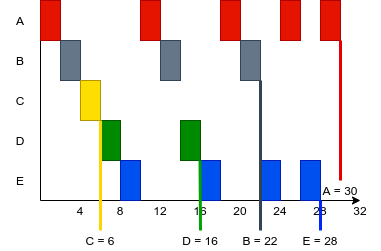
\includegraphics[keepaspectratio, width=\textwidth, height=\textheight]{img/rr.png} \\
            \end{figure}
		\end{minipage} \hfill \begin{minipage}{0.3\textwidth}
		\scalebox{0.8}{
            \begin{tabular}[t]{@{}cc@{}}
			\toprule
			Process & Turnaround  \\ 
			\midrule
			$A$ & 30 \\ 
			$B$ & 22 \\
			$C$ & 6 \\ 
			$D$ & 16 \\ 
			$E$ & 28 \\
			\bottomrule
		\end{tabular}
		}
        \end{minipage} \\ \vspace{0.7cm}
        \alert{\[\frac{102}{5} = 20.4 \] 
                \[ 20\text{ min } 24\text{ s} \]}
        
        \item Priority: $B = 5, E = 4, A = 3, C = 2, D = 1$ \\ \vspace{0.7cm}
        \begin{minipage}{0.49\textwidth}
            \begin{figure}
                    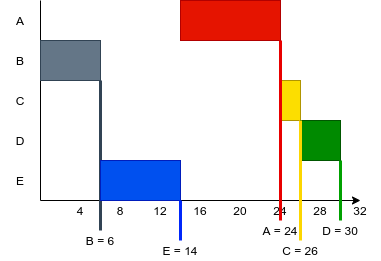
\includegraphics[keepaspectratio, width=\textwidth, height=\textheight]{img/priority.png} \\
                \end{figure}
        \end{minipage}\hfill \begin{minipage}{0.3\textwidth}
        \scalebox{0.8}{
        \begin{tabular}[t]{@{}cc@{}}
			\toprule
			Process & Turnaround \\
			\midrule
			$A$ & 24 \\ 
			$B$ & 6 \\
			$C$ & 26 \\ 
			$D$ & 30 \\ 
			$E$ & 14 \\
			\bottomrule
		\end{tabular}		
		}
        \end{minipage} \vspace{0.7cm}
		 \alert{\[ 20\text{ min}\]}
		 \framebreak
		 
		 \item FCFS \\ \vspace{0.7cm}
        \begin{minipage}{0.49\textwidth}
            \begin{figure}
                    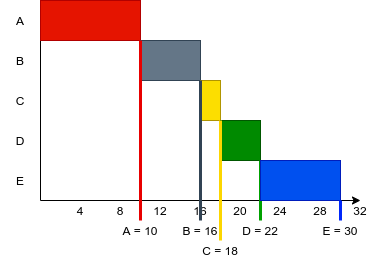
\includegraphics[keepaspectratio, width=\textwidth, height=\textheight]{img/fcfs.png} \\
                \end{figure}
        \end{minipage}\hfill \begin{minipage}{0.3\textwidth}
        \scalebox{0.8}{
        \begin{tabular}[t]{@{}cc@{}}
			\toprule
			Process & Turnaround \\
			\midrule
			$A$ & 10 \\ 
			$B$ & 16 \\
			$C$ & 18 \\ 
			$D$ & 22 \\ 
			$E$ & 30 \\
			\bottomrule
		\end{tabular}	
		}
        \end{minipage} \vspace{0.7cm}
		 \alert{\[ 19.2 = 19\text{ min } 12\text{ s} \]}
		 \framebreak
		 
		 \item SJF \\ \vspace{0.7cm}
        \begin{minipage}{0.49\textwidth}
            \begin{figure}
                    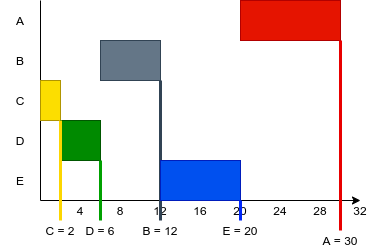
\includegraphics[keepaspectratio, width=\textwidth, height=\textheight]{img/sjf.png} \\
                \end{figure}
        \end{minipage} \hfill \begin{minipage}{0.3\textwidth}
        \scalebox{0.8}{
        \begin{tabular}[t]{@{}cc@{}}
			\toprule
			Process & Turnaround \\
			\midrule
			$A$ & 30 \\ 
			$B$ & 12 \\
			$C$ & 2 \\ 
			$D$ & 6 \\ 
			$E$ & 20 \\
			\bottomrule
		\end{tabular}
		}
        \end{minipage} \vspace{0.7cm}
		 \alert{\[ 14\text{ min} \]}
	\end{enumerate}
\end{frame}

\subsection*{Exercise 5}
\frame{\subsectionpage}
\begin{frame}[allowframebreaks, fragile]{Exercise 5}
	Consider the following \mintinline{c}{C} program:
	\begin{minted}[autogobble]{c}
    #define SIZE 1024*1024*1024 // 1GiB

    int main(void) {
        int array [SIZE];       

        return 0;
    }
	\end{minted}
	What happens when the program is executed? Why? 
	\begin{center}
	 \alert{Segmentation Fault: Stack Overflow. \\
	 Default stack size in Linux: \mintinline{bash}{ulimit -s} = 8192 KB.\footnote{Interesting read: \href{https://unix.stackexchange.com/questions/127602/default-stack-size-for-pthreads}{SO: Pages thread stacks}} \\}
	\end{center}
	\end{frame}

\subsection*{Exercise 6}
\frame{\subsectionpage}
\begin{frame}[allowframebreaks, fragile]{Exercise 6}
Write a program that accepts exactly one string as input and outputs the number of vowels (a, e, i, o, u, A, E, I, O, U) in it.
	If no or more than one command line argument is given, an error message should be displayed. \\
    \end{frame}
    \begin{frame}
    \adjustbox{varwidth=\textwidth}{%
    \inputminted[autogobble, fontsize=\tiny]{c}{code/ex6.c}
    }
    \end{frame}

    
\subsection*{Exercise 7}
\frame{\subsectionpage}
\begin{frame}[allowframebreaks, fragile]{Exercise 7}
\begin{enumerate}
		\item%
			Prove that Shortest-Job-First Scheduling always leads to the shortest average turnaround time,
			and is therefore optimal in that sense. \\
    \framebreak
            \textbf{Lemma 1~\autocite{tt}:} Given a set of jobs, moving a short job (S) before a long job (L) decreases the waiting time of the short job more than it increases that waiting time of the long job.
            Consequently the average turnaround time --- as well as the average waiting time -- decrease. \\
            \framebreak
            \textbf{Proof:} Let $L$, $S$ as above with run times $l$ and $s$ respectively. 
            $S1$ denotes the schedule before switching, while $S2$ denotes the schedule afterwards. The waiting time of $S$ with respect to schedule $S1$ is $WTS(S1)$. Define the others similarly. The total waiting time of $S, \ L$ with respect to a schedule is $WT_{Total}(S1) = WTS(S1) + WTL(S1)$, similarly for $S2$. \\
            Let $WTS(S2) = WTS(S1) - l$ the waiting time of $S$ without having to wait for $L$, i.e. when switching, while $WTL(S2) = WTL(S1) + s$ is the waiting time for $L$ in this case. \\
            \framebreak
            Using the above we get:
            \[ WT_{Total}(S1) > WT_{Total}(S2) \]
            \[ WTS(S1) + WTL(S1) > WTS(S2) + WTL(S2) \]
            \[ WTS(S1) + WTL(S1) > WTS(S1) - l + WTL(S1) + s \]
            \[ 0 > - l + s \]
            Since $l > s$, indeed $0 > - l + s$, thus $WT_{Total}(S1) > WT_{Total}(S2)$
			\hfill\qed \\
			\framebreak
			Applying the above Lemma repeatedly results in an ordering by runtime. With finitely many jobs and thus finitely many exchanges, this ordering is unique up to permutation of jobs with the same runtime and gives a shortest job first schedule. This schedule is minimal as there is no change that reduces the runtime further.
    \framebreak
		\item%
			This does not apply for different arrival times.
			Give a counter example. \\
			Five processes $A, B, C, D, E$ with runtimes $2, 4, 1, 1, 1$ and arrival times $0, 0, 3, 3, 3$. \\
			Initially only $A$ or $B$ can be selected. \\
			SJF gives $A, B, C/D/E$
			with an average turnaround time of \[ \frac{1}{5} (2 + 6 + 4 + 5 + 6) = 4.6 \]
			$C/D/E, A, B$ has the smaller average cycle time \[\frac{1}{5} (1 + 2 + 3 + 5 + 9) = 4 \]
	\end{enumerate}
\end{frame}
    
\section*{Exercise sheet 4}
\frame{\sectionpage}
\begin{frame}[allowframebreaks, fragile]{}
 \begin{figure}
           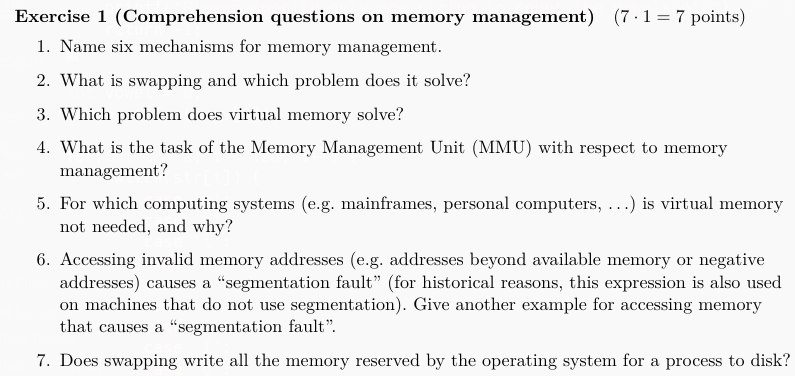
\includegraphics[keepaspectratio, width=\textwidth, height=\textheight-2\baselineskip-2\baselineskip]{img/100_ex4.png} \\
        \end{figure}
        \begin{itemize}
         \item Use the bold-printed keywords from chapter 3~\autocite{tanenbaum}, P. 187, P. 194, P. 196, P. 185 (also think of washing machines), P. 205,  what is paging good for
        \end{itemize}
        \framebreak
        
  \begin{figure}
          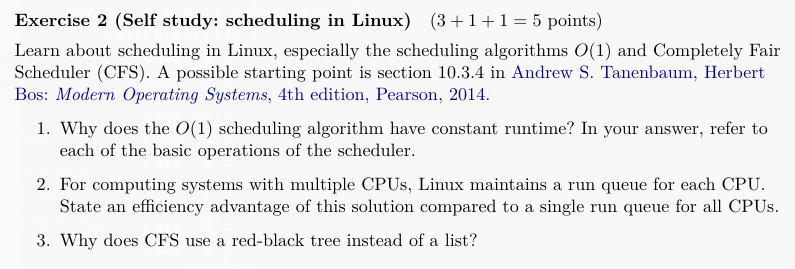
\includegraphics[keepaspectratio, width=\textwidth, height=\textheight-2\baselineskip-2\baselineskip]{img/101_ex4.png} \\
        \end{figure}
        \begin{itemize}
         \item Figure 10.10 in \autocite{tanenbaum}
         \item \href{https://www.cs.montana.edu/~chandrima.sarkar/AdvancedOS/CSCI560\_Proj\_main/index.html}{2.6 and ongoing}\footnote{https://www.cs.montana.edu/~chandrima.sarkar/AdvancedOS/CSCI560\_Proj\_main/index.html}
         \item \href{https://www.kernel.org/doc/html/latest/scheduler/sched-design-CFS.html}{TLDP - CFS Scheduler}\footnote{https://www.kernel.org/doc/html/latest/scheduler/sched-design-CFS.html}
        \end{itemize}
        \framebreak
        
         \begin{figure}
          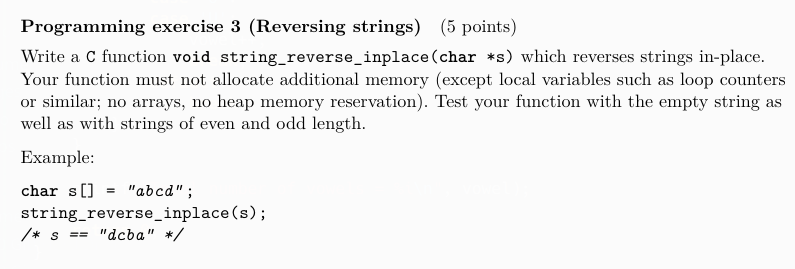
\includegraphics[keepaspectratio, width=0.8\textwidth, height=0.8\textheight-2\baselineskip-2\baselineskip]{img/102_ex4.png} \\
        \end{figure}
        \begin{itemize}
         \item Always swap two chars
         \item start at beginning and at end with exchange\\
         (1. Iter: change chars $0$ \& $n-1, \ \dots$)
         \item mind the \mintinline{c}{'\0'} null terminator of strings!
         \item Fix all warnings! \\
         \adjustbox{varwidth=\textwidth, scale = 0.7}{
         \mintinline{bash}{-g -fsanitize=undefined -fsanitize=address -Wall -Werror -Wpedantic -Wextra}
         }
        \end{itemize}
        \framebreak 
        
         \begin{figure}
          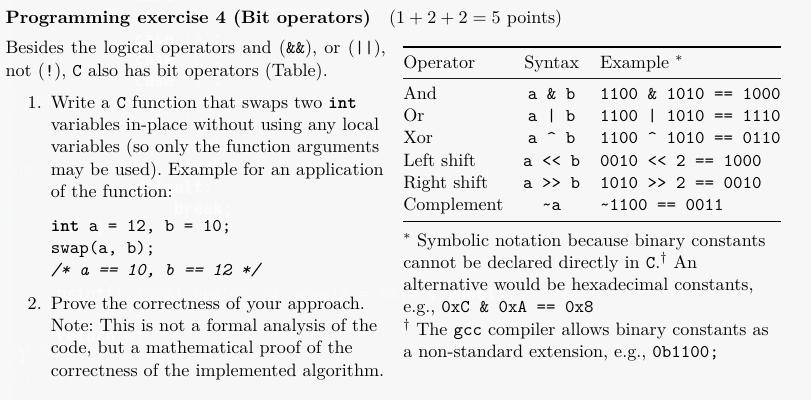
\includegraphics[keepaspectratio, width=\textwidth, height=\textheight]{img/103_ex4.png} \\
        \end{figure}
        \begin{itemize}
         \item xor is self-inverse: 
         \[ A \text{ XOR } B \text{ XOR } A = B \]
         \item You could start with 4.2
        \end{itemize}
        \framebreak 
        
        \begin{figure}
          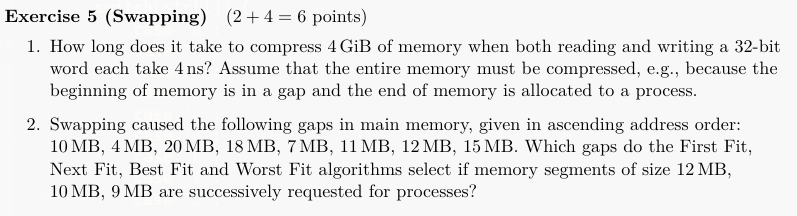
\includegraphics[keepaspectratio, width=0.8\textwidth, height=0.8\textheight-2\baselineskip-2\baselineskip]{img/104_ex4.png} \\
        \end{figure}
        \begin{itemize}
         \item 32-bit = 4 bytes. Every memory cell needs to be read and written
         \item Important, common exam exercise. \\ Understand the algorithms \& draw the memory per algorithm execution!
        \end{itemize}
        \framebreak 
        
        \begin{figure}
          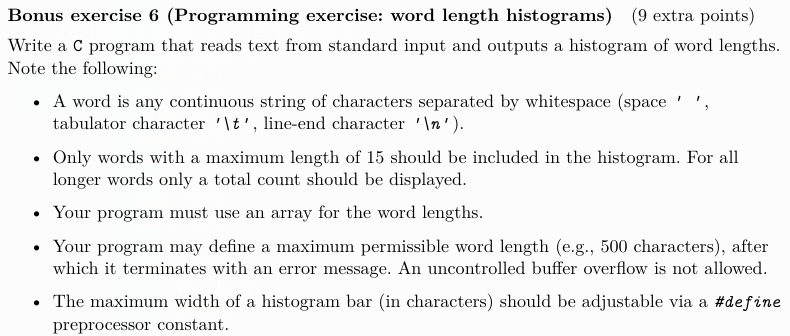
\includegraphics[keepaspectratio, width=0.8\textwidth, height=0.8\textheight-2\baselineskip-2\baselineskip]{img/105_ex4.png} \\
        \end{figure}
        \begin{itemize}
         \item Fix all warnings! \\
         \adjustbox{varwidth=\textwidth, scale = 0.7}{
         \mintinline{bash}{-g -fsanitize=undefined -fsanitize=address -Wall -Werror -Wpedantic -Wextra}
         }
         \item \href{https://en.cppreference.com/w/c/io/fscanf}{scanf} with \mintinline{c}{"%MAX_LENGTHs"}. 
         \item scale the histogram according to the most often encountered word length and the defined max length.
        \end{itemize}
\end{frame}

\frame{Syscall vs. Upcall vs. Hypercall \\
        Monotlithic vs. Micro vs. Hypervisor}

\section{References}
    \begin{frame}[allowframebreaks]
      \frametitle{References}
      \begin{tiny}
      \nocite{*}
      \printbibliography
      \end{tiny}
    \end{frame}


\end{document}
 
